\section{TrustAuditFlow 设计}

\subsection{与 BLoP 全节点模式的关系}

TrustAuditFlow 是 BLoP 全节点可信审计模式的轻量化扩展。BLoP 提供可信节点集合、事件监测、可信执行支持和 PBFT 风格确认过程。TrustAuditFlow 保留该模式作为高保障基线，并增加风险感知执行策略：高风险事件、争议事件和关键状态转移由完整可信节点集合确认，而常规且可批量处理的事件由可信审计委员会确认。

\begin{table}[t]
\centering
\caption{BLoP 全节点模式与 TrustAuditFlow 的关系。}
\label{tab:blop_relation}
\scriptsize
\begin{tabular}{p{1.45cm}p{2.55cm}p{2.55cm}}
\toprule
方面 & BLoP 全节点模式 & TrustAuditFlow 路径 \\
\midrule
确认者 & 所有可信节点 & 优先由可信委员会确认 \\
事件类型 & 高风险和争议事件 & 常规且可批量事件 \\
链上数据 & 事件状态记录 & 批量锚点和恢复状态 \\
回退机制 & 强安全基线 & 回退到全节点模式 \\
\bottomrule
\end{tabular}
\end{table}

这一关系对本文范围很重要。TrustAuditFlow 不是 BLoP 的弱替代品，而是在事件风险和频率使全节点确认成本相对较高时，为常规事件提供的附加路径。

\subsection{工作流}

图~\ref{fig:workflow} 展示了闭环审计恢复工作流。数据对象首先被分片并进行纠删码编码。系统随后计算分片哈希，构建 Merkle 根，并将对象承诺锚定到链上。审计者根据策略抽样链下分片。如果被挑战分片缺失、过期或与承诺不一致，系统记录异常，并检查剩余有效分片是否足以恢复。如果恢复成功，对象承诺和责任节点状态被更新。如果无法恢复或事件风险较高，则回退到全节点确认或外部仲裁。

\begin{figure*}[t]
\centering
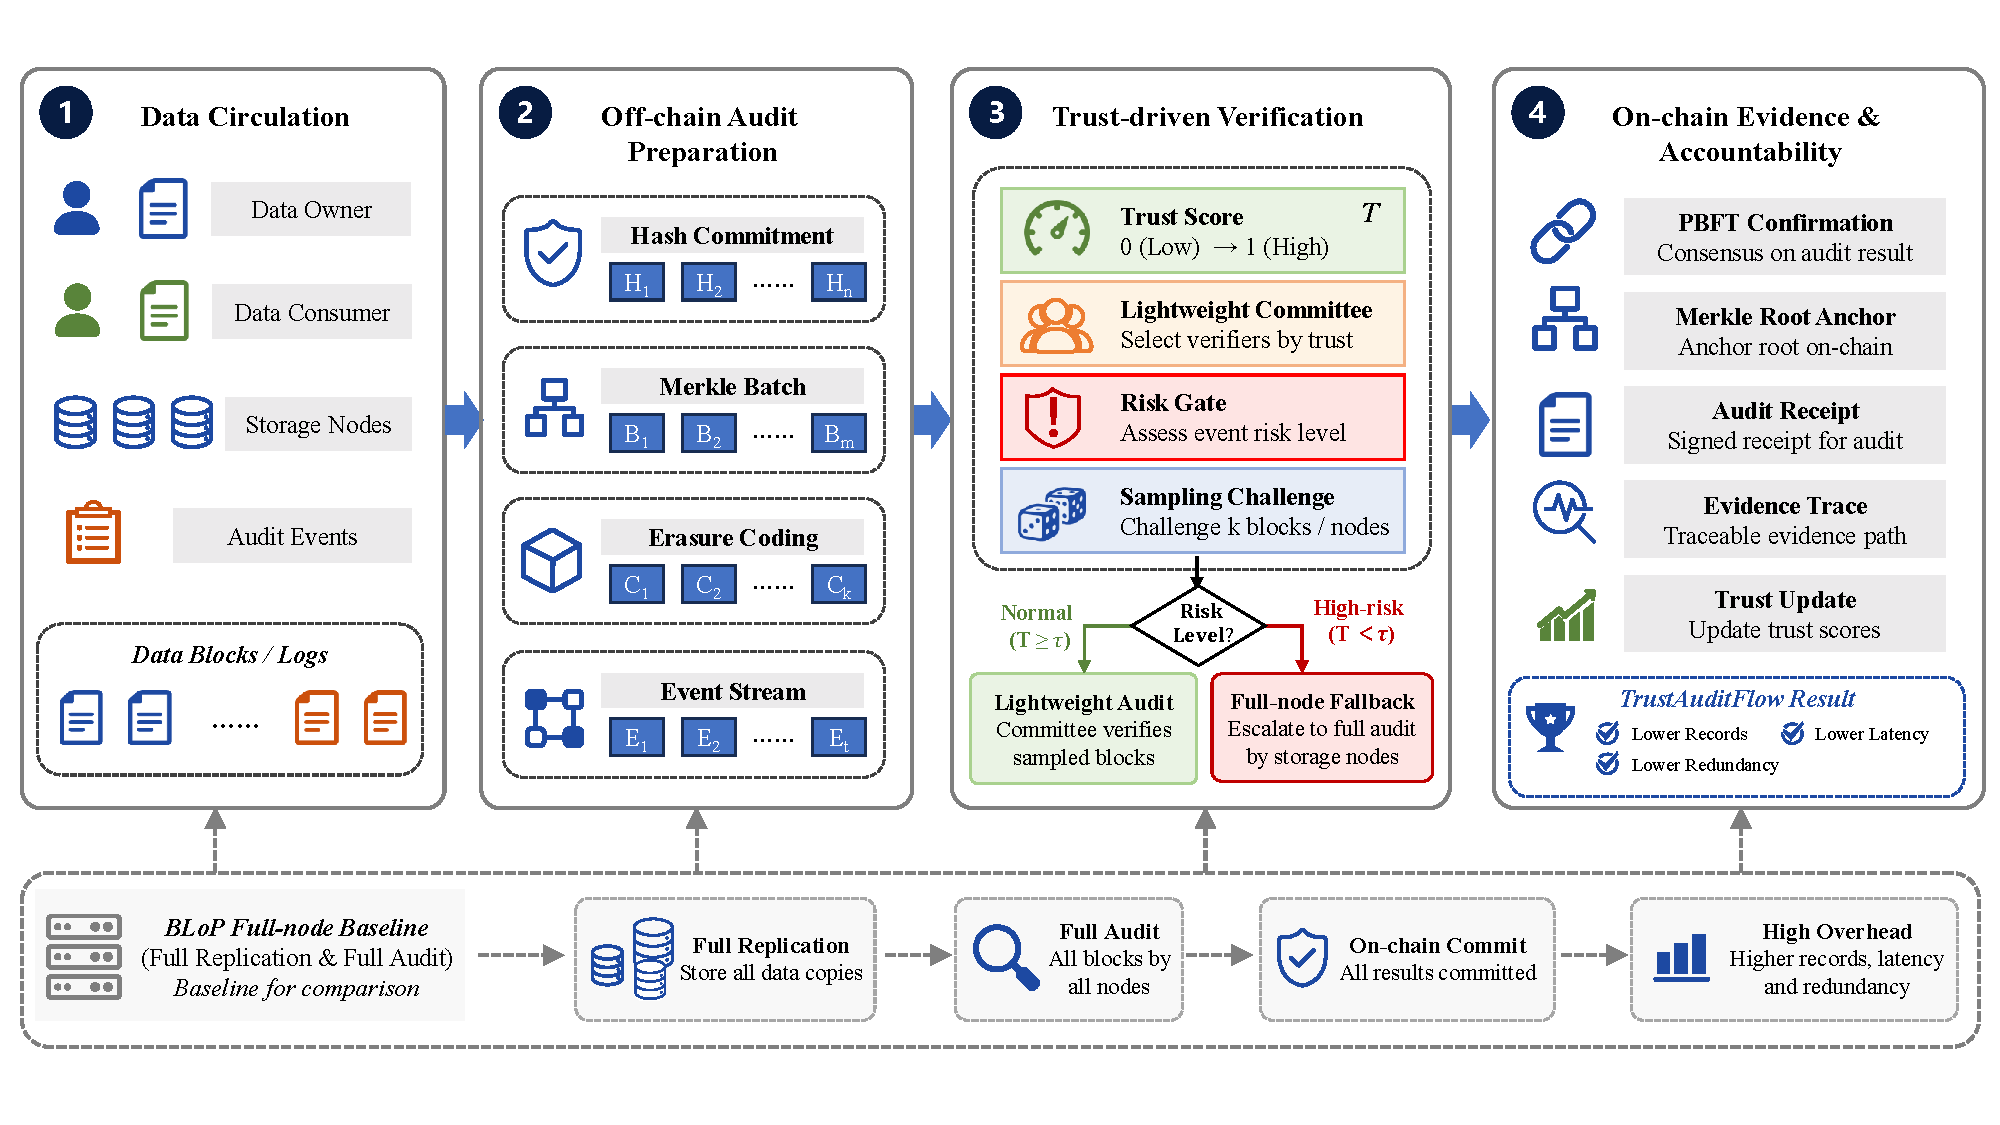
\includegraphics[width=\textwidth]{figures/trustauditflow_workflow.pdf}
\caption{TrustAuditFlow 工作流。}
\label{fig:workflow}
\end{figure*}

\subsection{信任分与委员会选择}

BLoP 通过可信计算和监测维护可信节点集合。TrustAuditFlow 复用这一思想，并将其转化为委员会选择规则。节点 $v_i$ 的信任分建模为
\begin{equation}
  T_i = \alpha A_i + \beta C_i + \gamma P_i,
\end{equation}
其中 $A_i$ 表示远程度量或配置状态，$C_i$ 表示历史审计行为和信用事件，$P_i$ 表示资源可用性。权重满足 $\alpha+\beta+\gamma=1$。

低于阈值 $\theta$ 的节点被排除出候选集合 $V_T$。对于具有策略 $policy_D$ 的数据对象，系统根据风险级别、审计频率和容错要求选择委员会 $C \subseteq V_T$。如果委员会容忍 $f$ 个拜占庭节点，则可用投票节点数量必须满足
\begin{equation}
  |C_{avail}| \geq 2f+1.
\end{equation}
如果该条件不满足，或对象被标记为高风险，则事件不通过轻量路径处理，而是升级到全节点确认。

\subsection{风险感知批量锚定}

TrustAuditFlow 区分常规事件和高风险事件。常规事件作为有序事件列表存储在链下。每当批量大小达到 $b$，系统构建 Merkle 根并向链上写入一个锚点。高风险事件使用更小批量、即时锚定或全节点回退。

对于 $n$ 个常规事件和批量大小 $b$，常规链上记录数量变为
\begin{equation}
  N_{chain} = \left\lceil \frac{n}{b} \right\rceil + N_{high},
\end{equation}
其中 $N_{high}$ 为需要单独处理的高风险事件数量。目标不是隐藏证据，而是将详细证据转移到链下，同时保留可验证链上摘要。

\subsection{抽样审计与异常生成}

给定审计策略，审计者抽样挑战集合 $Q=\{q_1,\ldots,q_r\}$。对于每个被挑战分片 $s_i$，存储节点根据校验模块返回分片、摘要或证明对象。哈希校验提供轻量完整性模块，同一接口也可以承载 PDP/PoR 校验。

如果校验失败，审计者产生异常事件
\begin{equation}
  e = \langle id_D, i, v_i, type, t, proof \rangle,
\end{equation}
其中 $type$ 表示分片缺失、哈希不匹配、超时、过期响应或证据不完整。该事件被追加到链下哈希链，并进入下一次锚定决策。

\subsection{纠删码恢复与信任更新}

当检测到异常集合 $F$ 时，系统检查剩余有效分片是否满足恢复阈值。对于 $(k,m)$ 纠删码配置，只要至少保留 $k$ 个有效分片，对象即可恢复。如果恢复成功，系统重新生成损坏分片，重新计算受影响分片哈希，并更新 Merkle 根。如果恢复失败，事件被标记为不可恢复并升级处理。

恢复或失败后，责任节点信任分被更新：
\begin{equation}
  T_i' = T_i - \lambda_1 I_{damage} - \lambda_2 I_{timeout} + \lambda_3 I_{recovered}.
\end{equation}
其中 $I_{damage}$、$I_{timeout}$ 和 $I_{recovered}$ 分别表示损坏、超时和成功协助恢复事件。该更新闭合治理循环：审计结果影响后续委员会选择。

\subsection{链上确认}

每个审计批次生成链上载荷，包含审计摘要、异常摘要、恢复状态、受影响节点、旧 Merkle 根、新 Merkle 根和链下证据哈希。委员会节点在 PBFT 风格法定人数规则下对载荷投票。已提交载荷更新对象状态和节点状态。如果委员会无法满足法定人数，或事件策略要求更强保障，则载荷被发送到全节点路径。

